\documentclass[12pt,a4paper]{article}

%------------------------------------------------
% Packages
%------------------------------------------------
\usepackage[T1]{fontenc}
\usepackage{lmodern}
\usepackage{graphicx}
\usepackage{amsmath,amssymb}
\usepackage{siunitx}
\usepackage{geometry}
\usepackage{fancyhdr}
\usepackage{booktabs}
\usepackage{caption}
\usepackage{float}
\usepackage{subcaption}
\usepackage{array}
\usepackage{setspace}
\usepackage[hidelinks]{hyperref}
\usepackage[backend=biber,style=numeric]{biblatex}

\addbibresource{references.bib}

%------------------------------------------------
% Page layout
%------------------------------------------------
\geometry{
    top=1in,
    bottom=1.2in,
    left=1in,
    right=1in
}

\setlength{\headheight}{15pt}
\setlength{\parskip}{0.4em}
\setlength{\parindent}{0pt}

\pagestyle{fancy}
\fancyhf{}
\fancyhead[L]{Ian Cullinane}
\fancyhead[R]{Newtonian cooling and adiabatic index}
\fancyfoot[C]{\thepage}

\sisetup{
    inter-unit-product = \cdot,
    uncertainty-mode = separate,
    per-mode = symbol
}

%------------------------------------------------
% Title
%------------------------------------------------
\title{
    \Large\textbf{Newtonian Cooling and the Adiabatic Index}\\[0.5em]
    \large PY2107 -- Experiment 4
}

\author{
    Ian Cullinane -- \textit{125413342}\\[0.5em]
    Lab Partner: Fionn Lichtsinn Doyle\\[0.5em]
    Demonstrators: Jonathan and Olivia
}

\date{21st October 2026}

\begin{document}

\maketitle
\thispagestyle{empty}

\newpage
\tableofcontents
\newpage

%================================================
\section{Abstract}
%================================================

This experiment investigates Newtonian cooling of a heated
calorimeter and determines the adiabatic index of air from the
oscillation period of a ball above an enclosed air volume. A linear
fit to the logarithm of the cooling temperature excess gives
$k=(1.465\pm0.007)\times10^{-4}\,\si{s^{-1}}$, corresponding to an
effective air boundary-layer thickness of
$b=(4.11\pm0.04)\,\si{mm}$. The oscillation measurements give
$\gamma=1.39\pm0.08$, consistent within uncertainty with the
diatomic ideal-gas prediction of $1.40$. The uncertainty in
$\gamma$ is dominated by the uncertainty in the mean oscillation
period.

%================================================
\section{Theory}
%================================================

\subsection{Newtonian Cooling}

When a hot object is surrounded by a cooler fluid, thermal energy
is transferred from the object to the surroundings. In this
experiment, the calorimeter loses heat to the surrounding air
\cite{py2107,incropera2018}.

The laboratory model assumes that heat is conducted through a thin
layer of approximately stationary air adjacent to the calorimeter.
Outside this boundary layer, convection carries the warmed air away
and replaces it with cooler air.

If the boundary layer has thickness $b$, the heat-transfer rate is
approximated by

\begin{equation}
    \dot{Q} =
    \frac{\lambda A}{b}(T-T_0),
    \label{eq:heatflow}
\end{equation}

where $\lambda$ is the thermal conductivity of air, $A$ is the
exposed surface area of the calorimeter, $T$ is its temperature,
and $T_0$ is the ambient temperature.

The model assumes that the temperature difference across the
boundary layer is approximately steady and that the calorimeter
and water can be represented by a single uniform temperature.

The rate of change of thermal energy of the calorimeter is related
to its temperature change by

\[
dQ = CdT,
\]

where $C$ is the total heat capacity. Since the object loses heat
when $T>T_0$, its energy balance is

\begin{equation}
    C\frac{dT}{dt}
    =-\frac{\lambda A}{b}(T-T_0).
    \label{eq:energybalance}
\end{equation}

Defining the temperature excess as

\[
\Theta=T-T_0,
\]
and assuming that the ambient temperature remains constant gives

\begin{equation}
    \frac{d\Theta}{dt}=-k\Theta,
    \label{eq:coolingode}
\end{equation}

where

\begin{equation}
    k=\frac{\lambda A}{bC}.
    \label{eq:kdef}
\end{equation}

Separating variables and integrating,

\[
\frac{d\Theta}{\Theta}=-k\,dt,
\]

gives

\[
\ln\Theta=-kt+\text{constant}.
\]
    
If the initial temperature at $t=0$ is $T_i$, then
$\Theta_i=T_i-T_0$, and the solution becomes

\begin{equation}
    \boxed{
    T(t)=T_0+(T_i-T_0)e^{-kt}
    }.
    \label{eq:newton}
\end{equation}

Therefore, the temperature difference between the calorimeter
and the surroundings decreases exponentially with time.

The characteristic cooling time is defined as

\[
\boxed{\tau=\frac{1}{k}}.
\]

A large value of $k$ corresponds to faster cooling, whereas a
small value corresponds to slower cooling.

Taking the natural logarithm of Eq.~\eqref{eq:newton} gives

\begin{equation}
    \boxed{
    \ln(T-T_0)=\ln(T_i-T_0)-kt
    }.
    \label{eq:logcooling}
\end{equation}

Thus, a graph of $\ln(T-T_0)$ against time should be linear, with
gradient $-k$. The cooling coefficient can therefore be obtained
from the negative gradient of a linear regression.

\subsection{Heating and Cooling Simultaneously}

During the heating phase, electrical energy is supplied to the
calorimeter while heat is simultaneously lost to the surroundings.

The electrical power supplied by the heater is

\begin{equation}
    P=VI,
    \label{eq:power}
\end{equation}

where $V$ is the voltage across the heater and $I$ is the current.

The energy balance during heating is

\[
C\frac{dT}{dt}=P-\frac{\lambda A}{b}(T-T_0).
\]

Using $k=\lambda A/(bC)$ gives

\begin{equation}
    \frac{dT}{dt}
    =\frac{P}{C}-k(T-T_0).
    \label{eq:heatingode}
\end{equation}

For constant power and ambient temperature, with initial
calorimeter temperature $T_i$, the solution is

\begin{equation}
    \boxed{
    T(t)-T_0
    =(T_i-T_0)e^{-kt}+\frac{P}{Ck}(1-e^{-kt})
    }.
    \label{eq:heatingsolution}
\end{equation}

This equation predicts that the temperature rises towards a
steady-state value when heating and cooling occur simultaneously.

If cooling is negligible over a short interval, the energy balance
reduces to

\[
C\frac{dT}{dt}=P=VI.
\]

Integrating gives

\[
\boxed{
T(t)=T_i+\frac{VI}{C}t
}.
\]
    
Consequently, the temperature should increase approximately
linearly during the initial stages of heating if the electrical
power is constant and heat losses are small.

In practice, deviations from linearity are expected because heat
is lost to the surroundings throughout the heating phase.

\subsection{Total Heat Capacity}

The total heat capacity is approximated by the sum of the heat
capacities of the aluminium calorimeter and the water:

\begin{equation}
    \boxed{
    C=mc_{\mathrm{Al}}+Mc_{\mathrm{water}}
    }.
    \label{eq:heatcapacity}
\end{equation}

Here, $m$ is the mass of the aluminium calorimeter, $M$ is the
mass of the water, and the specific heat capacities are

\begin{align}
    c_{\mathrm{Al}} &=
    \SI{900}{J.kg^{-1}.K^{-1}},\\
    c_{\mathrm{water}} &=
    \SI{4180}{J.kg^{-1}.K^{-1}}.
\end{align}

All masses must be expressed in kilograms. The resulting total
heat capacity has units of \si{J.K^{-1}}.

The stirrer and other components may also absorb heat. Their
contributions should be included if their heat capacities are
known and significant.

\subsection{Air Boundary-Layer Thickness}

Rearranging Eq.~\eqref{eq:kdef} gives the effective thickness of
the air boundary layer:

\begin{equation}
    \boxed{
    b=\frac{\lambda A}{kC}
    }.
    \label{eq:thickness}
\end{equation}

The thermal conductivity of dry air is taken to be

\begin{equation}
    \lambda=\SI{0.026}{W.m^{-1}.K^{-1}}.
\end{equation}

Once $A$, $k$, and $C$ have been measured or calculated, the
boundary-layer thickness can be determined.

The result represents an effective thickness within the simplified
heat-transfer model rather than a direct geometrical measurement
of the air surrounding the calorimeter.

\subsection{Adiabatic Index}

The adiabatic index of a gas is defined as the ratio of its
heat capacity at constant pressure to its heat capacity at
constant volume \cite{py2107}:

\begin{equation}
    \boxed{\gamma=\frac{C_P}{C_V}}.
\end{equation}

For an ideal gas undergoing an adiabatic process, no heat is
exchanged with the surroundings. The pressure and volume are
related by

\begin{equation}
    \boxed{PV^\gamma=\text{constant}}.
    \label{eq:adiabatic}
\end{equation}

In this experiment, the adiabatic index of air is determined by
measuring the period of oscillation of a steel ball or cylinder
inside a vertical tube connected to a vessel containing air.

The ball acts as a movable piston. Small vertical displacements
of the ball change the volume of the enclosed air, producing
pressure changes that provide a restoring force.

\subsection{Derivation of the Period of Oscillation}

Let $m$ be the mass of the ball, $A$ its cross-sectional area,
$V$ the equilibrium volume of the enclosed air, and $P$ the
equilibrium pressure of the enclosed air.

At equilibrium, the upward force due to the enclosed air balances
the atmospheric pressure acting downward and the weight of the
ball. Therefore,

\begin{equation}
    PA=P_{\mathrm{atm}}A+mg,
\end{equation}

which gives

\begin{equation}
    \boxed{P=P_{\mathrm{atm}}+\frac{mg}{A}}.
    \label{eq:equilibriumpressure}
\end{equation}

Now suppose the ball is displaced upwards by a small distance
$x$. The volume of the enclosed air increases by

\begin{equation}
    \Delta V=Ax.
\end{equation}

The new volume is therefore $V+Ax$. Assuming the oscillations
are sufficiently rapid to be adiabatic, Eq.~\eqref{eq:adiabatic}
gives

\begin{equation}
    P(V+Ax)^\gamma=P_0V^\gamma,
\end{equation}

where $P_0$ is the equilibrium pressure. Since $P_0=P$,

\begin{equation}
    P(x)=P\left(\frac{V}{V+Ax}\right)^\gamma.
\end{equation}

For small displacements, $Ax\ll V$, the binomial approximation
$(1+u)^{-\gamma}\approx1-\gamma u$ gives

\begin{equation}
    P(x)\approx P\left(1-\frac{\gamma Ax}{V}\right).
\end{equation}

Hence, the pressure change is

\begin{equation}
    \Delta P\approx-\frac{\gamma PA}{V}x.
\end{equation}

The resulting change in the upward force on the ball is
$A\Delta P$. The constant forces due to atmospheric pressure
and gravity cancel at equilibrium, so Newton's second law gives

\begin{equation}
    m\frac{d^2x}{dt^2}=A\Delta P.
\end{equation}

Substituting the pressure change,

\begin{equation}
    m\frac{d^2x}{dt^2}
    =-\frac{\gamma PA^2}{V}x.
\end{equation}

Rearranging,

\begin{equation}
    \boxed{
    \frac{d^2x}{dt^2}
    +\frac{\gamma PA^2}{mV}x=0
    }.
    \label{eq:shm}
\end{equation}

This is the equation of simple harmonic motion, with angular
frequency

\begin{equation}
    \omega^2=\frac{\gamma PA^2}{mV}.
\end{equation}

Since $\omega=2\pi/T$, where $T$ is the period of oscillation,

\begin{equation}
    \frac{4\pi^2}{T^2}
    =\frac{\gamma PA^2}{mV}.
\end{equation}

Rearranging gives the expression used to calculate the adiabatic
index:

\begin{equation}
    \boxed{
    \gamma=\frac{4\pi^2mV}{PA^2T^2}
    }.
    \label{eq:gamma}
\end{equation}

All quantities must be expressed in SI units:
$m$ in kilograms, $V$ in cubic metres, $P$ in pascals,
$A$ in square metres, and $T$ in seconds.

\subsection{Expected Value of the Adiabatic Index}

Air consists primarily of nitrogen and oxygen, which are
diatomic molecules. At ordinary temperatures, a diatomic ideal
gas has three translational and two rotational degrees of
freedom. Vibrational degrees of freedom are approximately
inactive at these temperatures.

The equipartition theorem gives the molar heat capacity at
constant volume as

\begin{equation}
    C_V=\frac{f}{2}R,
\end{equation}

where $f$ is the number of active degrees of freedom and $R$
is the molar gas constant.

For a diatomic gas, $f=5$ \cite{py2107}, so

\begin{equation}
    C_V=\frac{5}{2}R.
\end{equation}

For an ideal gas,

\begin{equation}
    C_P-C_V=R.
\end{equation}

Therefore,

\begin{equation}
    C_P=\frac{7}{2}R,
\end{equation}

and the expected adiabatic index is

\begin{equation}
    \boxed{
    \gamma_{\mathrm{theory}}
    =\frac{C_P}{C_V}
    =\frac{7}{5}=1.40
    }.
\end{equation}

This value provides the theoretical reference against which
the experimental result can be compared.

\newpage

%================================================
\section{Experimental Procedure}
%================================================

\subsection{Newtonian Cooling}

The apparatus consisted of an aluminium calorimeter, water, a
stirrer, an electrical heating coil, a power supply, a digital
ammeter and voltmeter, two thermometers, a balance, and a
computer-based temperature recording system.

The first thermometer recorded the temperature of the
calorimeter and water, while the second thermometer measured the
ambient-air temperature. Allowing us to dynamically calculate $\Delta T$

The mass $m$ of the empty metal calorimeter was measured
using a balance. The curved surface area $A$ of its walls was
also determined.

The calorimeter was approximately half-filled with water.
The mass $M$ of the water was measured, ensuring that the
heating coil was covered.

The lid was fitted, with the thermometer in contact with
the water. The apparatus was allowed to settle before the
initial water and ambient-air temperatures were recorded.

The heating circuit was connected to the power supply.
The ammeter range was checked to ensure that its maximum
reading was set to \SI{10}{A} or less. The electrical power
was calculated using $P=VI$.

The water was stirred gently before readings to maintain
a reasonably uniform temperature. Care was taken to prevent
the stirrer from touching the heating coil.

The LoggerPro software was set up to take measurements 
every 12 seconds.

After 30 minutes, the heating circuit was disconnected.
Temperature measurements continued at 12 second intervals
during cooling for an hour and a half.

\subsection{Adiabatic Index}

The apparatus consisted of a large vessel containing enclosed
air, a precision vertical glass tube, and a cylinder that fitted 
closely inside the tube.

The apparatus was checked to ensure that the tap was
closed and that the protective mat was positioned at the
bottom of the vessel.

The ball was carefully dropped into the glass tube,
allowing it to oscillate vertically on the enclosed air
cushion.

The motion was recorded using a camera's slow-motion mode and
analysed to determine the oscillation period. The elapsed time
measured from the footage was divided by 8 to convert it to real
time, accounting for the camera's slow-motion factor.

The time taken for a number of complete oscillations
was measured. The period was calculated by dividing the
total measured time by the number of oscillations.

Several measurements were taken to obtain repeated
estimates of the period. The number of oscillations used
for each measurement was chosen so that the period could
be determined accurately.

The mass, cross-sectional area, and enclosed air
volume were obtained from the experimental apparatus or
measurements. The equilibrium pressure was calculated
using Eq.~\eqref{eq:equilibriumpressure}. Ambient air 
pressure was taken from the surface pressure charts for 
that day, see Fig.~\ref{fig:surface_pressure}.

The adiabatic index was calculated from the measured
period using Eq.~\eqref{eq:gamma}.

The ball and tube were handled carefully because the fit between
them was precise. Dirt or thermal expansion of the ball could
affect its motion and introduce systematic errors.

\begin{figure}[H]
\centering
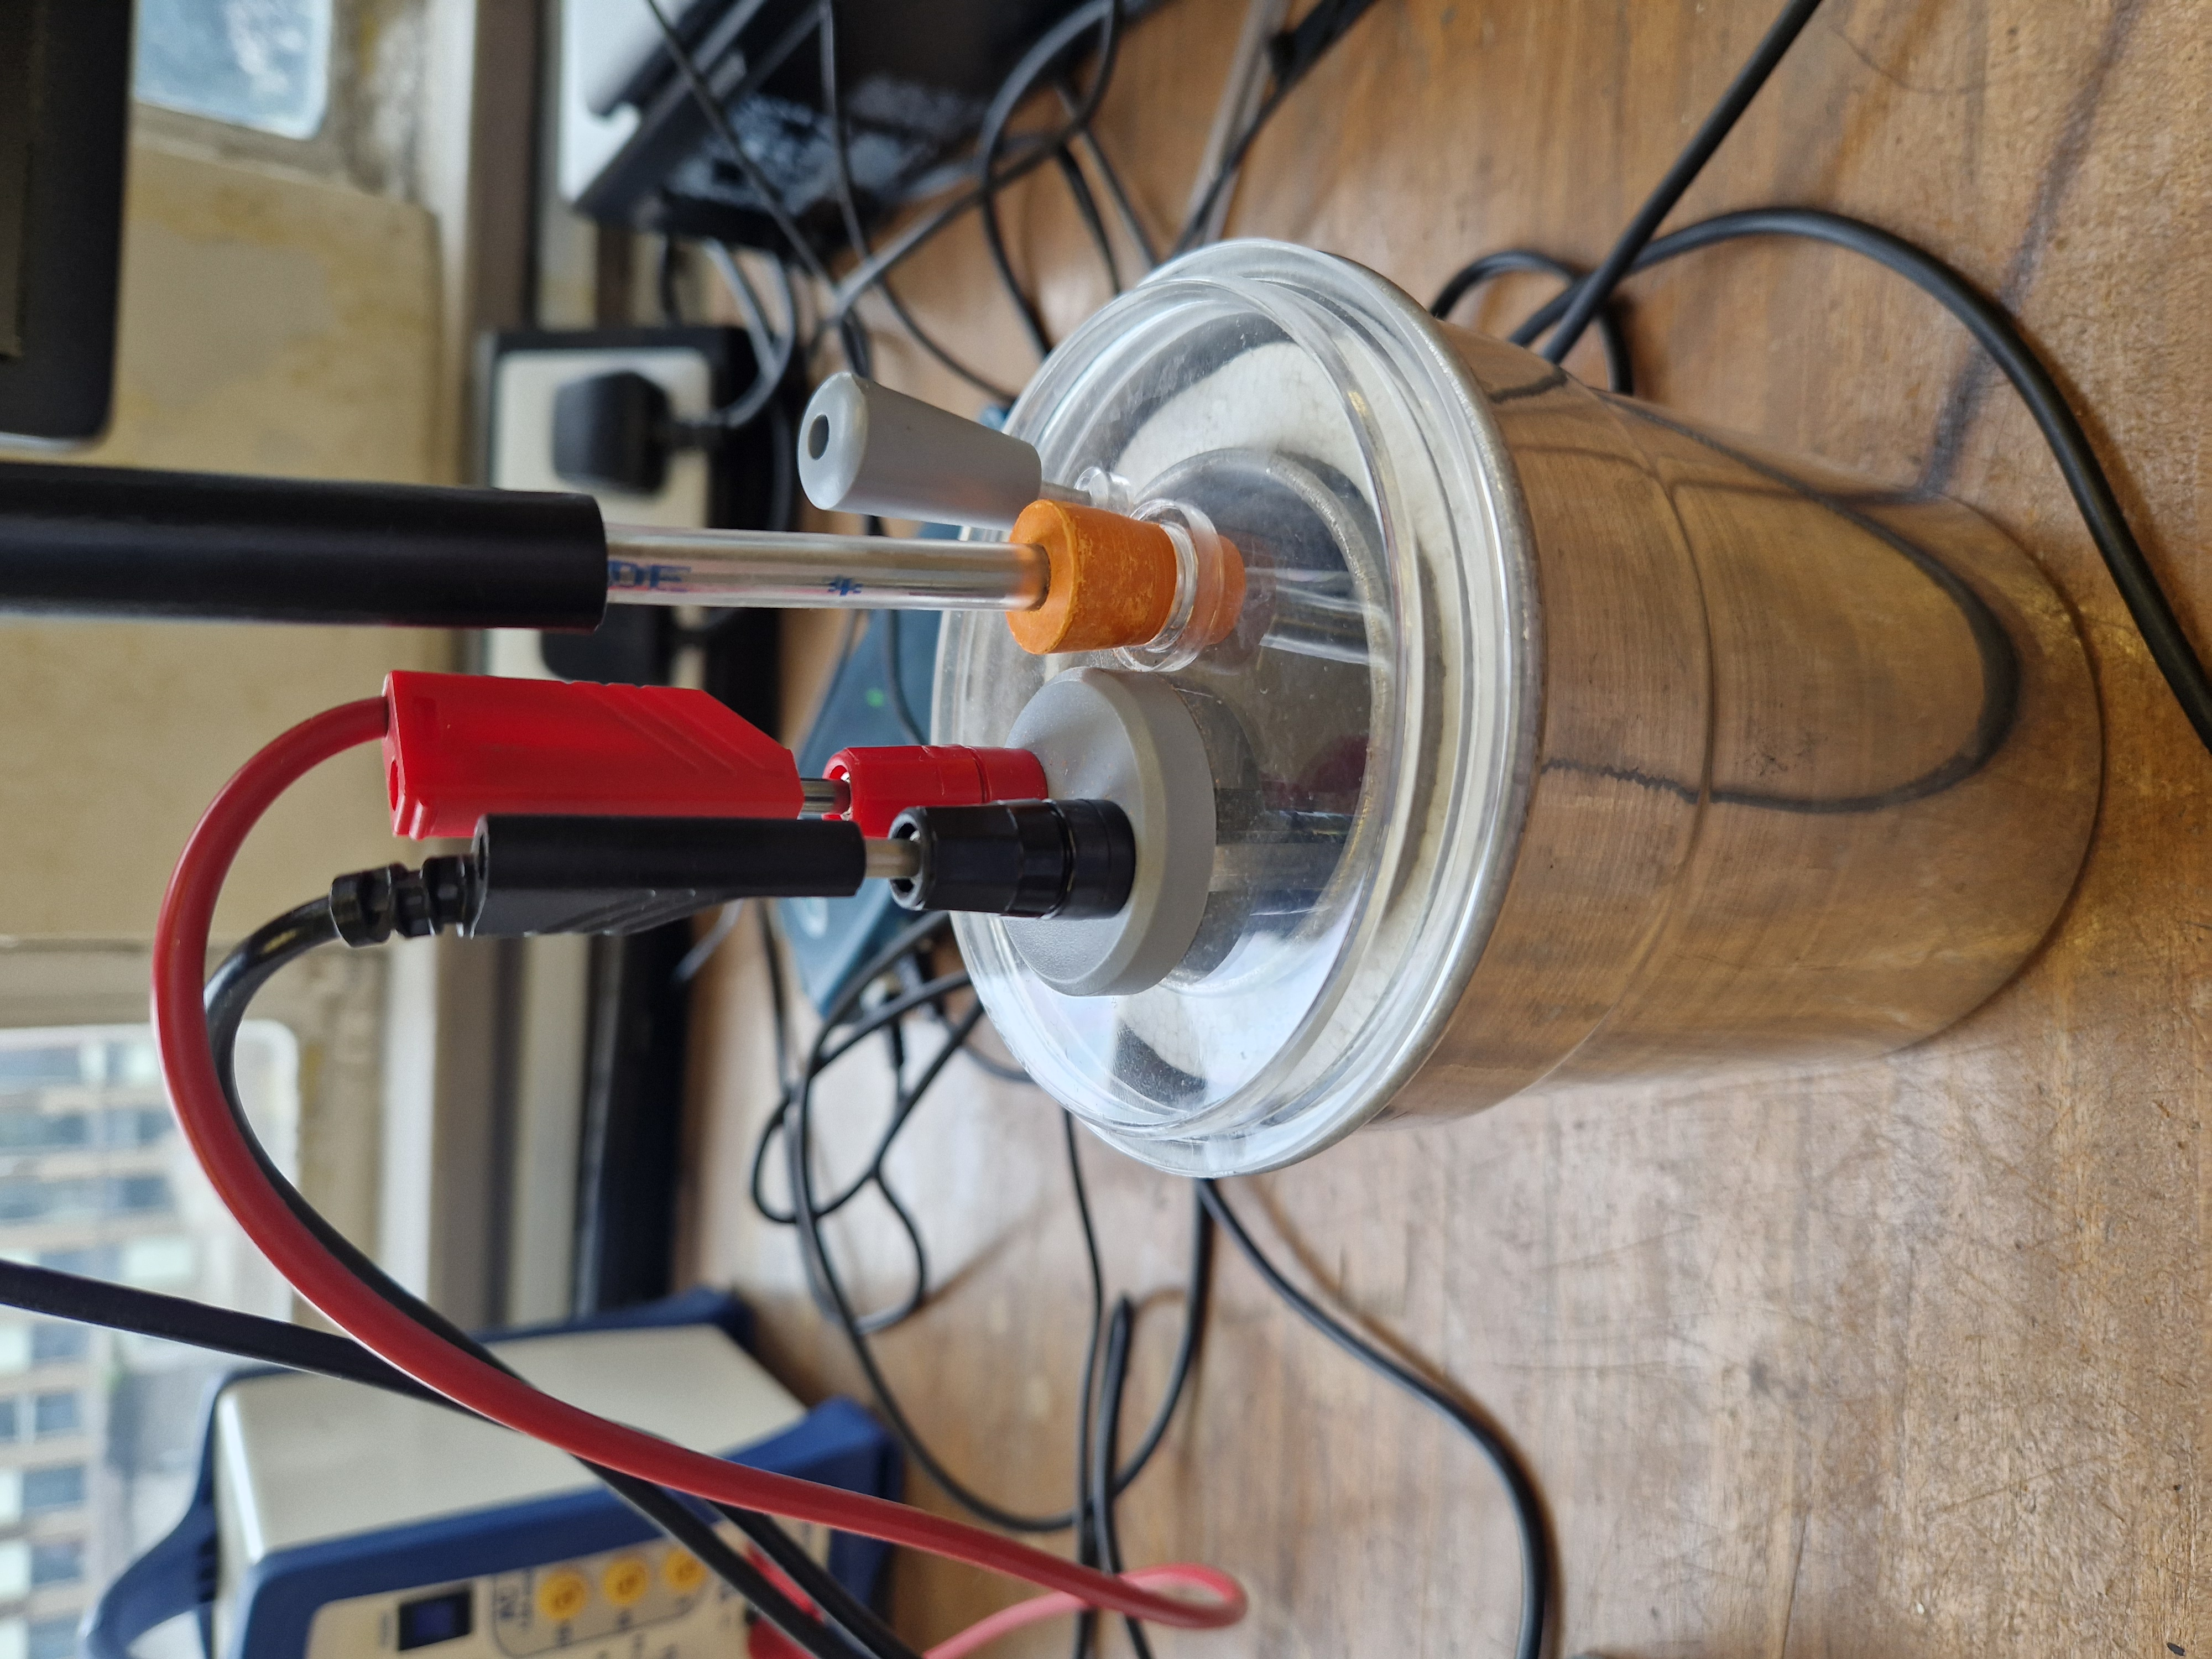
\includegraphics[angle=-90,width=0.8\textwidth]{images/Calorimeter_Apparatus.jpg}
\caption{Calorimeter apparatus used in the experiment.}
\label{fig:calorimeter_apparatus}
\end{figure}

\begin{figure}[H]
    \centering
    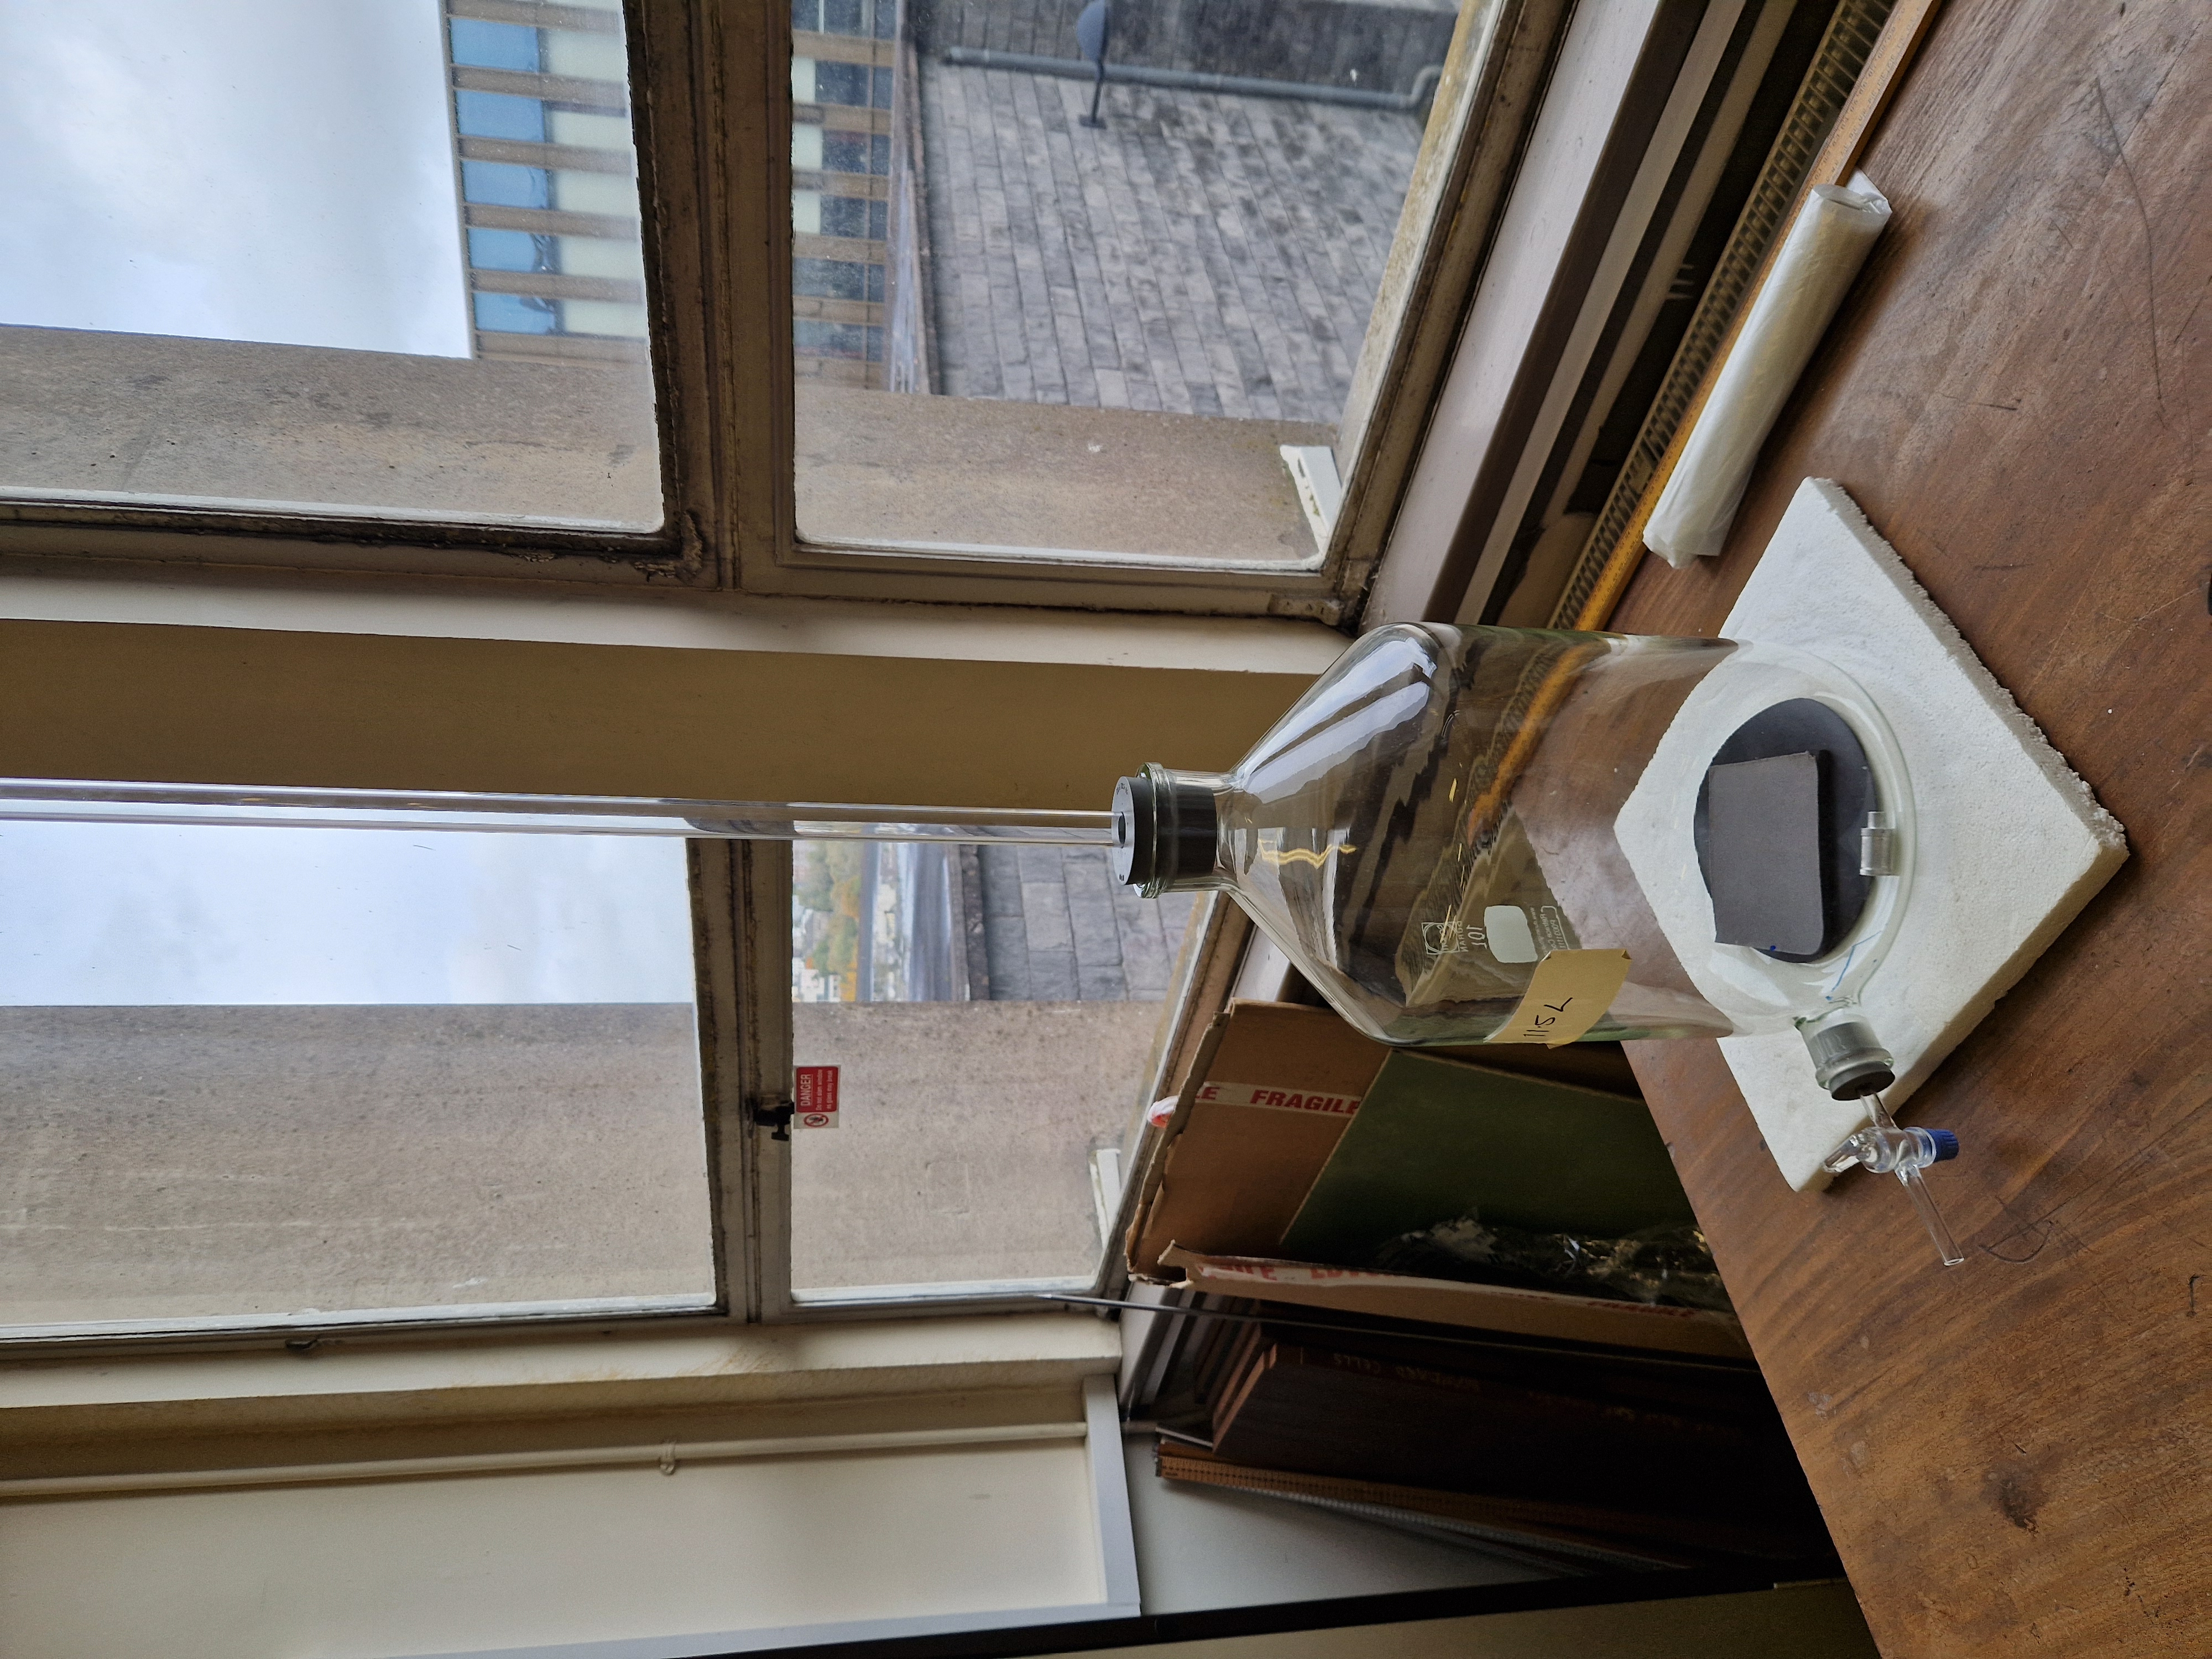
\includegraphics[angle=-90, width=0.8\textwidth]{images/Adiabatic_Apparatus.jpg}
    \caption{Adiabatic apparatus used in the experiment.}
    \label{fig:adiabatic_apparatus}
\end{figure}

\newpage

%================================================
\section{Results}
%================================================

\subsection{Measured Quantities}

The measured quantities used in the analysis are summarised
in Table~\ref{tab:measurements_k}.

\begin{table}[H]
\centering
\caption{Measured quantities used to calculate $k$.}
\label{tab:measurements_k}
\begin{tabular}{lll}
\toprule
Quantity & Symbol & Measured value\\
\midrule
Mass of empty calorimeter & $m$ & $\si{0.003489 \pm 0.0000005}{kg}$ \\
Mass of water & $M$ & $\si{0.150061 \pm 0.000005}{kg}$ \\
Curved surface area & $A$ & $\si{0.0145947 \pm 0.000001}{m^2}$\\
Supply voltage & $V$ & $\si{2.98 \pm 0.005}{V}$\\
Heating current & $I$ & $\si{1.25 \pm 0.000005}{A}$\\
\bottomrule
\end{tabular}
\end{table}

\begin{table}[H]
\centering
\caption{Parameters required to calculate $\gamma$.}
\label{tab:measurements_gamma}
\begin{tabular}{lll}
\toprule
Quantity & Symbol & Value\\
\midrule
Mass of ball & $m$ & $\si{0.01482 \pm 0.0000005}{kg}$\\
Cross-sectional area & $A$ & $\si{0.000201 \pm 0.000001}{m^2}$\\
Enclosed air volume & $V$ & $\si{0.01 \pm 0.0001}{m^3}$\\
Atmospheric pressure & $P_{\mathrm{atm}}$ & $\si{99600 \pm 50}{Pa} $\\
Equilibrium pressure & $P$ & $\si{100323.3 \pm 50}{Pa} $\\
Mean oscillation period & $\bar{T}$ & $\si{1.017 \pm 0.03}{s} $\\
\bottomrule
\end{tabular}
\end{table}

\subsection{Temperature-Time Graph}

Figure~\ref{fig:temperature} shows the measured temperature
difference against elapsed time during the cooling period.

\begin{figure}[H]
    \centering
    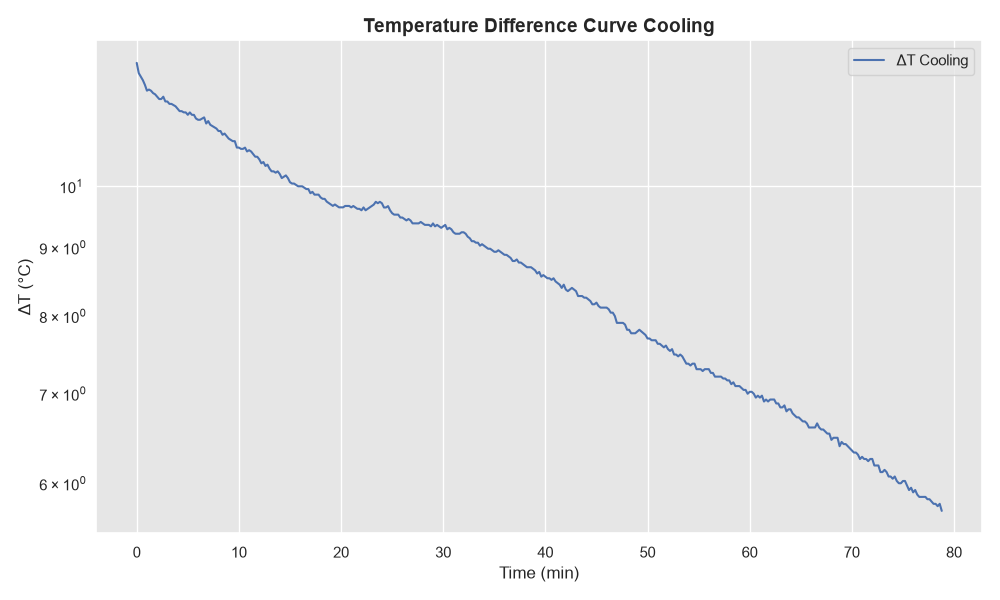
\includegraphics[width=0.9\textwidth]{images/Temperature_Difference_Curve_Cooling.png}
    \caption{Calorimeter temperature difference as a function of elapsed time for cooling period. Logarithmic scale used for the temperature difference to show linear relationship.}
    \label{fig:temperature}
\end{figure}

\newpage

%================================================
\section{Analysis}
%================================================

\subsection{Electrical Power}

The electrical power supplied to the heater is calculated using

\begin{equation}
    P=VI.
\end{equation}

For example, the calculation using the measured values is

\begin{equation*}
    P=(2.98)(1.25)
      =3.725\ \si{W}.
\end{equation*}

The current was stable as a result of the low voltage and thus temperature.

\subsection{Total Heat Capacity}

Using Eq.~\eqref{eq:heatcapacity},

\begin{equation}
    C=mc_{\mathrm{Al}}+Mc_{\mathrm{water}}.
\end{equation}

Substituting the measured masses,

\begin{align*}
    C = (0.0035)(\SI{900}{J.kg^{-1}.K^{-1}}) + (0.15)(\SI{4180}{J.kg^{-1}.K^{-1}}) = 630.4 \si{J.K^{-1}}.
\end{align*}

\subsection{Heating-Rate Comparison}

Figure~\ref{fig:heating-rate} compares the measured temperature
excess with a linear fit, a no-loss reference, and the constant-power
model including Newtonian cooling. For the latter, $P=VI$ and $C$
are calculated from the measured electrical and calorimeter
parameters, while $k$ is taken from the cooling-phase fit; the
model starts at the first measured heating excess. With
$I=\SI{1.25}{A}$, the no-loss heating rate is
$VI/C=5.909\times10^{-3}\,\si{K.s^{-1}}$, while the measured
linear-fit slope is $4.701\times10^{-3}\,\si{K.s^{-1}}$.
The lower rate is consistent with heat loss during heating. The
cooling-aware curve is the more appropriate ideal prediction for
the full heating interval, although its constant-$k$, constant-power
assumptions and the structured residuals limit how closely it should
be expected to match every measurement.

\begin{figure}[H]
    \centering
    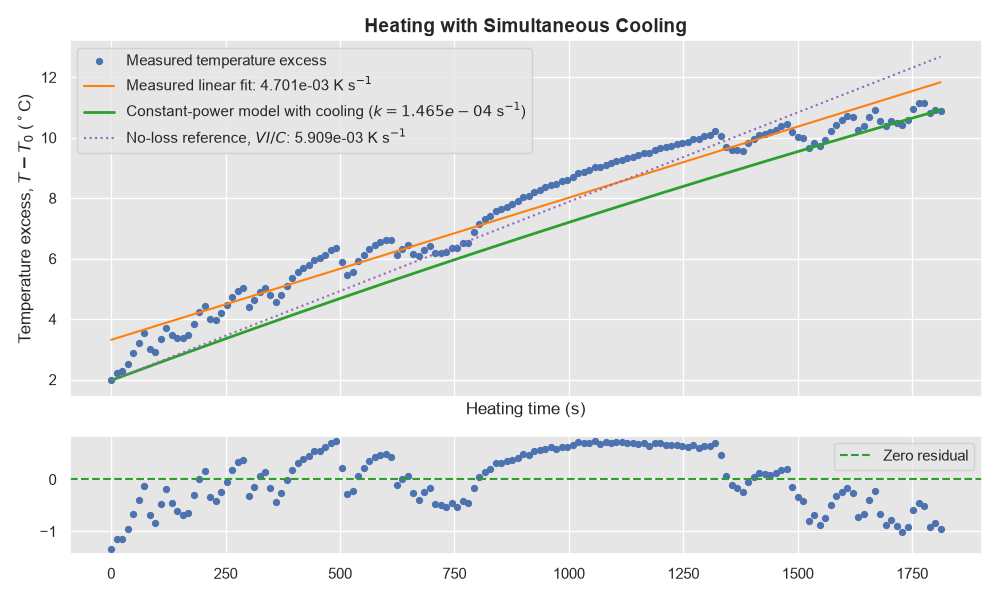
\includegraphics[width=0.9\textwidth]{images/Heating_With_Cooling.png}
    \caption{Measured heating temperature excess compared with a
    linear fit, the constant-power Newton-cooling model using the
    measured cooling coefficient, and a no-loss reference. The lower
    panel shows residuals from the cooling-aware model.}
    \label{fig:heating-rate}
\end{figure}

\subsection{Cooling Coefficient}

Let $t_c$ denote the time measured from when the heater was
switched off. For every cooling measurement, calculate the
temperature excess

\begin{equation}
    \Theta=T-T_0.
\end{equation}

Then calculate $\ln(\Theta)$ for measurements with $\Theta>0$.

Plotting $\ln(T-T_0)$ against $t_c$. From Eq.~\eqref{eq:logcooling} 
yields a straight line with slope $-k$ as seen in Fig.~\ref{fig:cooling-log-fit}.

The graph yielded

\[
    k = (1.465 \pm 0.007) \times 10^{-4}\ \si{s^{-1}}, \quad 
    \tau = \frac{1}{k} = (6829 \pm 33)\ \si{s}.
\]

A suitable linear fit should be selected by examining the graph
and residuals. Measurements very close to ambient temperature
may be unreliable because small temperature errors produce
large relative errors in $T-T_0$.

\begin{figure}[H]
    \centering
    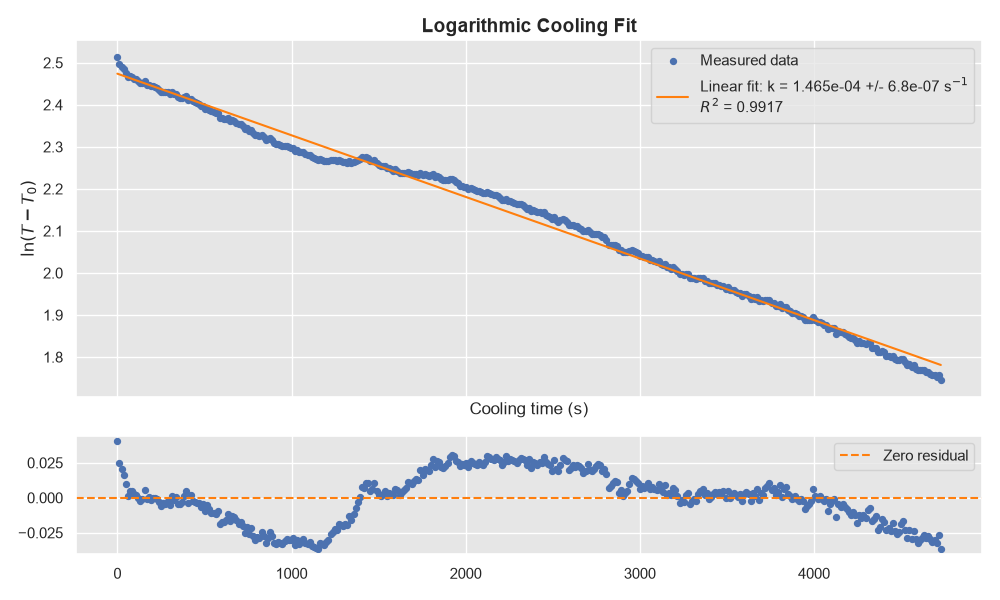
\includegraphics[width=0.9\textwidth]{images/Cooling_Log_Linear_Fit.png}
    \caption{Natural logarithm of the cooling temperature excess
    against time, with the linear regression used to determine $k$.}
    \label{fig:cooling-log-fit}
\end{figure}

\begin{figure}[H]
    \centering
    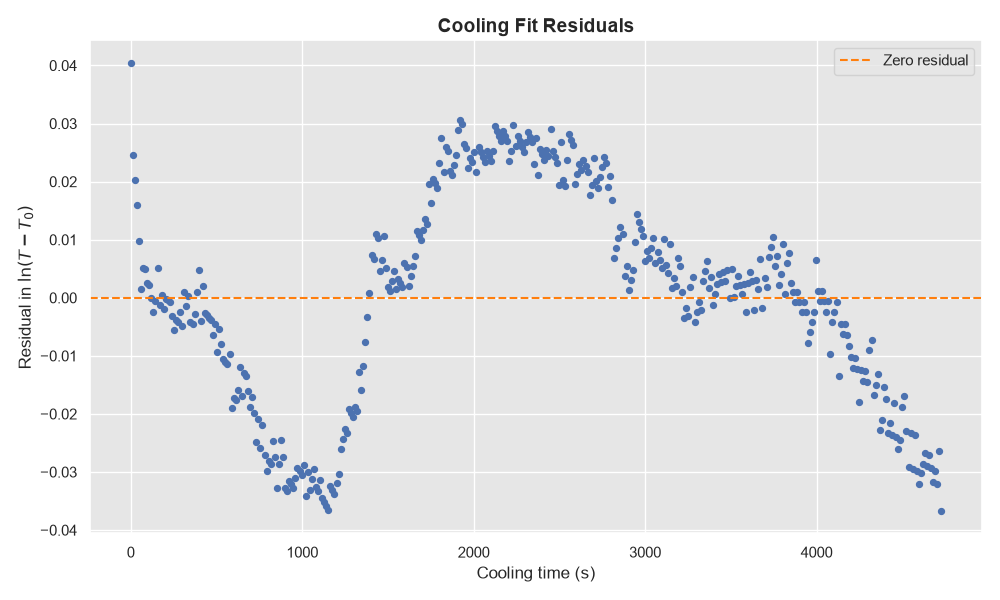
\includegraphics[width=0.9\textwidth]{images/Cooling_Log_Residuals.png}
    \caption{Residuals from the logarithmic cooling fit. A pattern
    in the residuals indicates departures from a single-exponential
    cooling model.}
    \label{fig:cooling-residuals}
\end{figure}

The residuals from the full-record fit show systematic structure
rather than random scatter. Therefore, the high $R^2$ value alone
does not establish that a single exponential describes the complete
cooling interval. The fitted slope uncertainty accounts for
regression scatter, but not this model limitation; the fit interval
should be checked before treating the resulting $k$ as definitive.

\subsection{Approximate Linear Cooling Method}

For sufficiently small $kt_c$, the exponential may be expanded
using a Taylor series:

\begin{equation}
    e^{-kt_c}\approx 1-kt_c.
\end{equation}

Therefore,

\begin{equation}
    T_{\mathrm{cool}}(t_c)
    \approx T_{\max}-(T_{\max}-T_0)kt_c.
\end{equation}

A graph of temperature against cooling time is consequently
approximately linear over a sufficiently short interval.

If its gradient is $g$, then

\begin{equation}
    g\approx-k(T_{\max}-T_0),
\end{equation}

and hence

\begin{equation}
    \boxed{
    k\approx-\frac{g}{T_{\max}-T_0}
    }.
\end{equation}

This is an approximation. The logarithmic fit is the more direct
method for estimating $k$ from the exponential cooling model.

\subsection{Boundary-Layer Thickness}

Using Eq.~\eqref{eq:thickness},

\begin{equation}
    b=\frac{\lambda A}{kC}.
\end{equation}

Substituting the thermal conductivity of air and the measured
and calculated quantities gives

\begin{equation*}
    b=(4.11 \pm 0.04) \si{mm}.
\end{equation*}

\subsection{Adiabatic Index}

Using Eq.~\eqref{eq:gamma} with the mean period and apparatus
parameters in Table~\ref{tab:measurements_gamma},

\begin{align*}
    \gamma
    &=\frac{4\pi^2(0.01482)(0.010)}
    {(100323.3)(0.000201)^2(1.01737)^2}\\
    &=1.395\approx1.39.
\end{align*}

The uncertainty in this value is propagated from the measured
quantities in the Error Analysis section, giving
$\gamma=1.39\pm0.08$.

\subsection{Fluid Simulation}

A supplementary finite-difference fluid simulation was conducted
to illustrate buoyancy-driven flow and heat transfer around a
cooling calorimeter. It uses a pressure-projection flow solver,
explicit temperature advection and diffusion, and a lumped
calorimeter energy balance. The simulation is qualitative context;
it was not used to calculate the experimental results.

\subsubsection{Analytic estimate from geometry}

The geometry does permit an analytic estimate. The flow is
buoyancy-driven, so the Rayleigh number is the controlling
parameter rather than the Reynolds number:
$\mathrm{Ra}_H=g\beta\Delta T H^3/(\nu\alpha)$.
For air at the film temperature ($\nu=1.6\times10^{-5}$,
$\alpha=2.25\times10^{-5}\,\si{m^2.s^{-1}}$, $\mathrm{Pr}=0.71$,
$\beta=1/T_f$) and an initial excess $\Delta T\approx12.3\,\si{K}$,
$\mathrm{Ra}_H\approx1.3\times10^{6}$. The Churchill--Chu correlation
for a vertical surface \cite{incropera2018},

\[
    \mathrm{Nu}_H=\left\{0.825+\frac{0.387\,\mathrm{Ra}_H^{1/6}}
    {\left[1+(0.492/\mathrm{Pr})^{9/16}\right]^{8/27}}\right\}^2
    \approx 17.7,
\]

gives $h=\mathrm{Nu}_H\lambda/H\approx4.4\,\si{W.m^{-2}.K^{-1}}$ and an
effective conductive layer thickness

\[
    b_{\mathrm{theory}}=\frac{\lambda}{h}=\frac{H}{\mathrm{Nu}_H}
    \approx5.9\,\si{mm}.
\]

As the calorimeter cools to $\Delta T\approx6\,\si{K}$ this rises to
about $7\,\si{mm}$. This is directly comparable to the experimental
$b=(4.11\pm0.04)\,\si{mm}$, since both are defined by
$b=\lambda/h$: the analytic value is approximately $44$--$70\%$
larger. Plausible
causes are the neglected radiative loss, the lid and base
contributing to heat loss (the experiment's $A$ covers only the
curved wall), the assumed $H$, and the approximate air
properties. The Churchill--Chu result also carries roughly
$\pm10$--$20\%$ correlation uncertainty. The analytic natural-convection
estimate provides a separate correlation-based comparison, not a
validation of the simulation or a direct prediction of the
experimental cooling coefficient.

\subsubsection{Simulation diagnostics}

For the reported run, the time step was $dt=0.1$. The code returned
$T_{\mathrm{cal}}=43.55$, a mean fluid temperature of $20.10$, and
a peak speed of $0.01758$, all in the model's grid-based units.
The corresponding diagnostics were
$\mathrm{Re}_{\mathrm{peak}}=5.624$,
$\mathrm{Pr}=3.333$, $\mathrm{Gr}=38592$,
$\mathrm{Ra}=128641$, and a grid-based Nusselt estimate of
$18.889$. The reported thermal boundary-layer diagnostic was
$1.899$ grid units, and the fitted cooling time constant was
$11.82$ simulation-time units.

These are diagnostics of the numerical run, not measurements of
the laboratory apparatus. In particular, the grid-based thermal
boundary-layer diagnostic is not the effective conduction
thickness $b=\lambda/h$ inferred from the experiment, and the
simulation has no dimensional calibration to metres or seconds.

\subsubsection{Convective heat loss and qualitative analysis}

Figs. \ref{fig:convective_heat_loss} and \ref{fig:sim} show the
convective heat loss and Newton cooling curves for the calorimeter.
The simulation illustrates heat transfer accompanied by
buoyancy-driven flow. It does not establish that the simulation
quantitatively reproduces the laboratory cooling curve.

\begin{figure}[H]
\centering
\includegraphics[width=0.8\textwidth]{images/sim.png}
\caption{Convective heat loss from the calorimeter.}
\label{fig:convective_heat_loss}
\end{figure}

\begin{figure}[H]
\centering
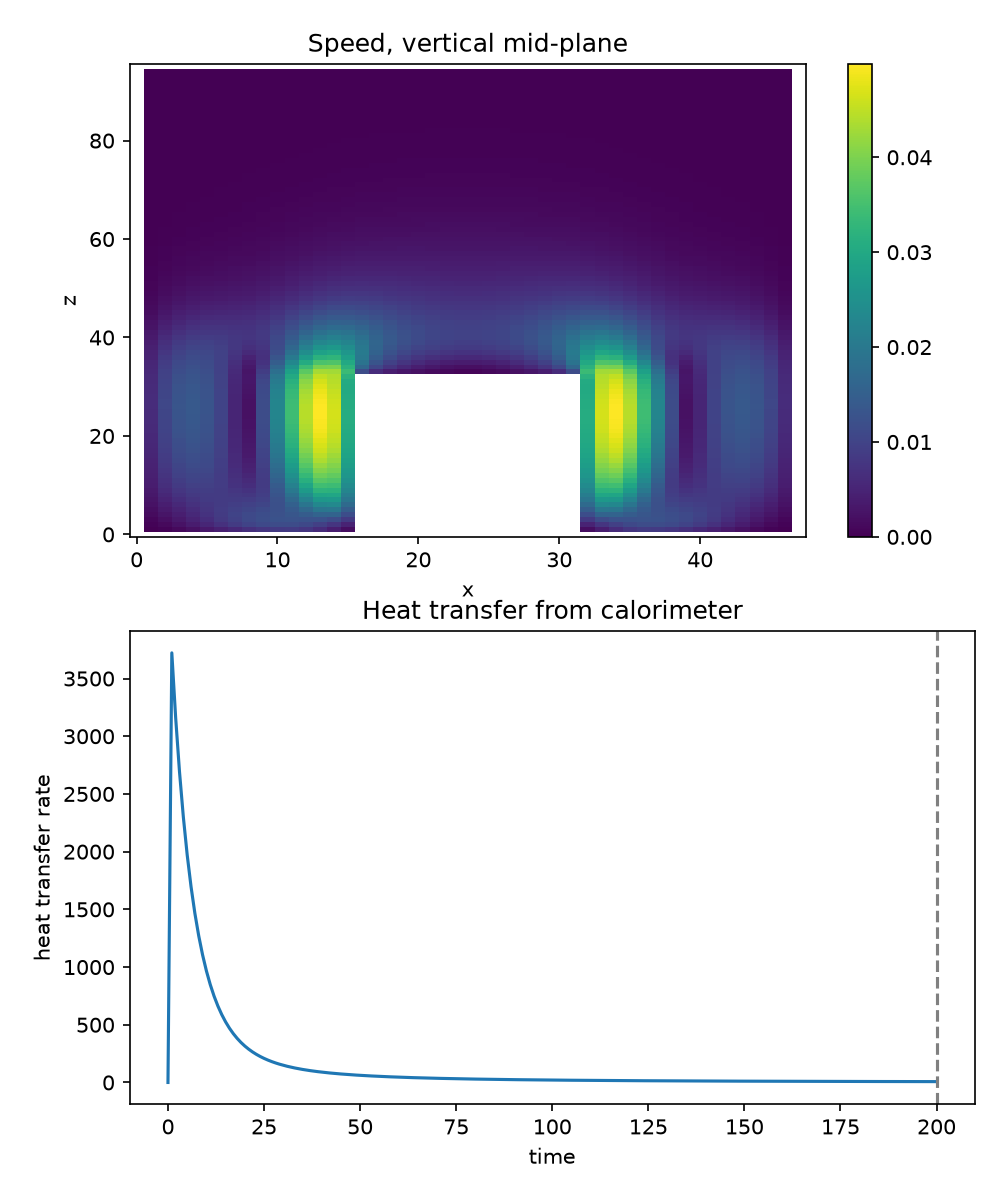
\includegraphics[width=0.8\textwidth]{images/Sim_curve.png}
\caption{Simulation of convective heat loss from the calorimeter.}
\label{fig:sim}
\end{figure}

\newpage

%================================================
\section{Error Analysis}
%================================================

The principal sources of uncertainty in the cooling analysis are
the mass measurements, the calorimeter surface area, the
temperature readings, the ambient temperature, and the fitted
cooling coefficient.

The uncertainty in $k$ directly affects the inferred boundary-layer
thickness.

For independent uncertainties,

\begin{equation}
    \left(\frac{\sigma_b}{b}\right)^2
    =
    \left(\frac{\sigma_A}{A}\right)^2+
    \left(\frac{\sigma_k}{k}\right)^2+
    \left(\frac{\sigma_C}{C}\right)^2,
\end{equation}

where uncertainty in $\lambda$ has been neglected.

The uncertainty in heat capacity is

\begin{equation}
    \sigma_C=
    \sqrt{
    (c_{\mathrm{Al}}\sigma_m)^2+
    (c_{\mathrm{water}}\sigma_M)^2
    }.
\end{equation}

The absolute uncertainty in the boundary-layer thickness is then

\begin{equation}
    \boxed{
    \sigma_b=b
    \sqrt{
    \left(\frac{\sigma_A}{A}\right)^2+
    \left(\frac{\sigma_k}{k}\right)^2+
    \left(\frac{\sigma_C}{C}\right)^2
    }
    }.
\end{equation}

\begin{equation*}
    \boxed{b=(4.11 \pm 0.04) \si{mm}}.
\end{equation*}

Other sources of systematic error include heat transfer through
the lid and supports, imperfect mixing of the water, sensor
response time, and the assumption that the boundary layer has
a constant thickness.

\subsection{Adiabatic Index}

Assuming independent uncertainties in the quantities in
Eq.~\eqref{eq:gamma}, propagation of uncertainty gives

\begin{equation}
    \left(\frac{\sigma_\gamma}{\gamma}\right)^2
    =
    \left(\frac{\sigma_m}{m}\right)^2+
    \left(\frac{\sigma_V}{V}\right)^2+
    \left(\frac{\sigma_P}{P}\right)^2+
    \left(2\frac{\sigma_A}{A}\right)^2+
    \left(2\frac{\sigma_{\bar{T}}}{\bar{T}}\right)^2.
\end{equation}

Using the uncertainties in Table~\ref{tab:measurements_gamma}
gives $\sigma_\gamma\approx0.084$, so the result is reported as

\begin{equation*}
    \boxed{\gamma=1.39\pm0.08}.
\end{equation*}

Here, the uncertainty in the mean period is the standard error
of the six measured periods. It is the dominant contribution to
the propagated uncertainty; the result does not include additional
systematic uncertainty from the camera's slow-motion calibration
or departures from the ideal adiabatic model.

\newpage

%================================================
\section{Discussion}
%================================================

The measurements test two separate models: exponential cooling
of a calorimeter and approximately adiabatic compression of air
by an oscillating piston. A small numerical natural-convection
model was also explored as a side project. It helps illustrate a
possible flow mechanism during cooling, but it was not part of
the laboratory requirements and is not used to calculate the
experimental results.

\subsection{Heating Phase}

For constant electrical power and negligible heat loss, the
expected initial heating rate is

\begin{equation}
    \frac{dT}{dt}=\frac{VI}{C}.
\end{equation}

The measured fit gives $4.701\times10^{-3}\,\si{K.s^{-1}}$,
compared with the no-loss prediction
$5.909\times10^{-3}\,\si{K.s^{-1}}$. The measured rate is about
20\% lower. This is consistent with heat being lost while the
calorimeter is heated; structured residuals also show that a
single straight line is only an approximate description of the
full heating record. The current is recorded as \SI{1.25}{A},
consistent with the power calculation. Its stated uncertainty is
retained from the measurement table, although its very small size
should be checked against the instrument specification.

\subsection{Cooling Phase}

Newtonian cooling predicts an exponential decrease in the
temperature difference between the calorimeter and its
surroundings \cite{py2107,incropera2018}. The fit gives
$k=(1.465\pm0.007)\times10^{-4}\,\si{s^{-1}}$, corresponding to
$\tau=6829\pm33\,\si{s}$. This uncertainty describes the
regression fit, not every source of experimental uncertainty.

Although the logarithmic graph is broadly linear, its residuals
show systematic structure. Thus, the fit supports an
exponential-like trend over the measured interval, but does not
establish that one cooling constant describes the entire record.
Changes in ambient temperature, multiple heat-transfer paths,
and non-uniform calorimeter temperature are plausible
contributors. The reported uncertainty should be understood as
a statistical fit uncertainty, with additional model uncertainty
not quantified here.

\subsection{Boundary-Layer Thickness}

The resulting $b=(4.11\pm0.04)\,\si{mm}$ follows from the
single-layer conduction approximation and the fitted $k$. It is
an effective model parameter, not a direct measurement of the
fluid's local thermal boundary-layer profile. Its small quoted
uncertainty does not include uncertainty in the assumptions of
uniform temperature, constant ambient conditions, or the chosen
heat-transfer model.

\subsection{Adiabatic Index}

The measured value, $\gamma=1.39\pm0.08$, is consistent within
uncertainty with the diatomic ideal-gas value of $1.40$ from
equipartition theory \cite{py2107}. The difference is only
$0.006$, much smaller than the propagated uncertainty. The
uncertainty is dominated by the spread in the measured periods.
The camera's slow-motion calibration, enclosed-volume and
tube-area measurements, and possible friction or leakage around
the ball may add systematic effects not included in that
propagation.

\subsection{Supplementary Natural-Convection Simulation}

The accompanying simulation is a separate numerical
demonstration of cooling from a hot, vertical cylindrical
calorimeter. It uses a pressure-projection flow solver, explicit
temperature advection and diffusion, and a lumped-temperature
calorimeter energy balance \cite{cullinane2026simulation}.
The closed outer walls are no-slip and thermally insulated; heat
passes between the calorimeter and fluid. The model illustrates
buoyancy-driven flow during cooling, but is not evidence that
the simulation quantitatively reproduces the laboratory cooling
curve. Its run diagnostics are summarised in
Appendix~\ref{tab:simulation-diagnostics}.

\subsection{Limitations}

The main limitations of the experiment include:

\begin{itemize}
    \item Changes in ambient temperature, sensor uncertainty,
    imperfect mixing, and heat loss through the calorimeter lid
    and supports.
    \item Structured residuals in the heating and cooling fits,
    which indicate that the simple models do not describe every
    measurement equally well.
    \item The uniform-temperature and constant-effective-layer
    assumptions in the calorimeter analysis.
    \item Timing and slow-motion calibration uncertainty, as
    well as possible friction or leakage in the oscillation
    apparatus.
    \item For the supplementary simulation, no dimensional
    calibration, grid/time-step convergence tests, or validation
    against a benchmark or the measured cooling data. The
    explicit thermal scheme and idealised geometry also limit
    quantitative conclusions.
\end{itemize}

The experimental uncertainty estimates account for selected
measurement scatter, but not all systematic or model errors.
Likewise, the simulation is best treated as qualitative context
until its convergence and physical calibration have been
established.

\newpage

%================================================
\section{Conclusion}
%================================================

This experiment investigated Newtonian cooling of a heated
calorimeter and determined the adiabatic index of air from the
oscillation of a ball above an enclosed air volume.

The cooling fit yielded
$k=(1.465\pm0.007)\times10^{-4}\,\si{s^{-1}}$ and an effective
air-layer thickness of $b=(4.11\pm0.04)\,\si{mm}$. The
oscillation analysis gave $\gamma=1.39\pm0.08$, consistent with
the diatomic ideal-gas prediction of $1.40$. The uncertainty in
$\gamma$ is dominated by the measured period spread, while
systematic timing and apparatus effects remain possible.

The measured heating rate was approximately 20\% below the
constant-power, no-loss prediction, as expected when heat loss
occurs during heating. Systematic residual structure in both the
heating and cooling analyses cautions against interpreting the
quoted fit uncertainties as complete uncertainty budgets.

As a side project, the fluid simulation provided a qualitative
example of buoyancy-driven flow coupled to calorimeter cooling:
the reported run produced non-zero flow while the calorimeter
cooled to a model temperature of $43.55$. Its grid-based
diagnostics cannot be compared directly with the laboratory
measurements, so it supplements rather than changes the
experimental conclusions. A dimensional mapping, convergence
study, and validation would be needed before making quantitative
claims from that model.

%================================================
\section{References}
%================================================

\printbibliography

%================================================
\appendix
%================================================

\section{Appendix}

\subsection{Results}

For each trial, if $N$ complete oscillations take a measured
slow-motion video time $t_{\mathrm{video}}$, the real-time period
is

\begin{equation}
    \boxed{T=\frac{t_{\mathrm{video}}}{8N}}.
\end{equation}

The factor of 8 converts the video time to real time. The measured
video times, oscillation counts, and calculated periods are
recorded in Table~\ref{tab:periods}.

\begin{table}[H]
    \centering
    \caption{Measured oscillation periods.}
    \label{tab:periods}
    \begin{tabular}{cccc}
    \toprule
    Trial &  Video time, $t_{\mathrm{video}}$ (\si{s})
    & Number of oscillations, $N$
    & Period, $T$ (\si{s})\\
    \midrule
    1 & 26.04 & 3 & 1.085 \\
    2 & 52.45 & 7 & 0.936607 \\
    3 & 60.45 & 8 & 0.944531\\
    4 & 77.62 & 10 & 0.97025\\
    5 & 34.73 & 4 & 1.08531\\
    6 & 25.98 & 3 & 1.0825\\
    \bottomrule
    \end{tabular}
\end{table}

\subsection{Weather conditions}

\begin{figure}[H]
    \centering
    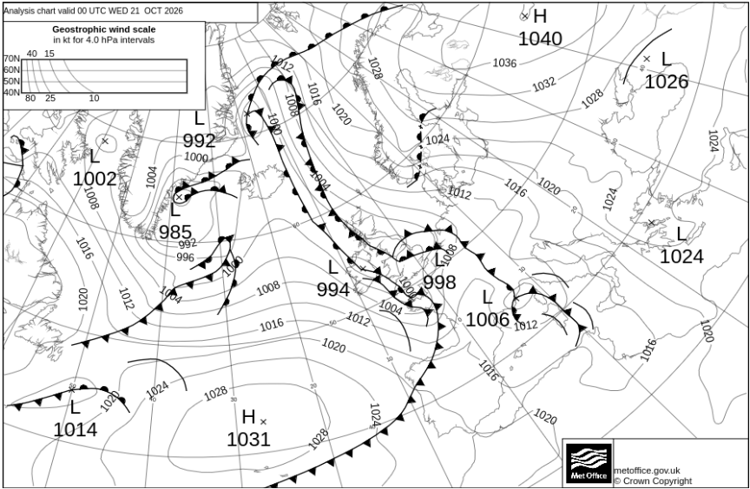
\includegraphics[width=0.8\textwidth]{images/Surface_pressure_chart.png}
    \caption{Surface pressure chart showing the weather conditions during the experiment.}
    \label{fig:surface_pressure}
\end{figure}

\subsection{Supplementary simulation: model and run}

This simulation was an optional side project, not a requirement
of the laboratory briefing. The implementation uses a
finite-difference pressure-projection method for flow and advances
the thermal field using explicit upwind advection and face-based
diffusion. The calorimeter has a spatially uniform temperature
and loses heat exchanged at its fluid-facing cells. The outer
walls are stationary and impermeable, and thermally insulated.
This is a simplified natural-convection model; the code is cited
as the implementation source \cite{cullinane2026simulation}.

The reported run used $dt=0.1$. Its other configuration
parameters are not specified here, so the diagnostics below are
reported as returned by the simulation rather than as a
reproducible benchmark. Values are in grid-based or
nondimensional units unless otherwise noted.

\begin{table}[H]
    \centering
    \caption{Diagnostics returned by the reported supplementary
    simulation run.}
    \label{tab:simulation-diagnostics}
    \begin{tabular}{ll}
    \toprule
    Diagnostic & Value\\
    \midrule
    Time step, $dt$ & 0.1\\
    Calorimeter temperature & 43.5549\\
    Mean fluid temperature & 20.1032\\
    Maximum speed & $1.7576\times10^{-2}$\\
    Peak Reynolds number, $\mathrm{Re}$ & 5.624\\
    Prandtl number, $\mathrm{Pr}$ & 3.333\\
    Grashof number, $\mathrm{Gr}$ & 38592.3\\
    Rayleigh number, $\mathrm{Ra}$ & 128640.9\\
    Grid-based Nusselt estimate, $\mathrm{Nu}$ & 18.889\\
    Thermal boundary-layer diagnostic & 1.899 grid units\\
    Cooling time constant & 11.815 simulation-time units\\
    Relative thermal energy & 34678.32\\
    \bottomrule
    \end{tabular}
\end{table}

The thermal boundary-layer value is a grid-based diagnostic, not
a measurement of the experimental boundary layer or of the
effective thickness $b=\lambda/h$. The relative thermal energy
is an internal numerical diagnostic, not a substitute for
convergence or validation testing.

\end{document}